

\begin{frame}{Requerimientos de biblioteca de Stack} 
    \begin{itemize}
        \item Protocolo LIFO (El primero que entra es el primero que sale)
        \item El tamano de el stack debe ser configurable por el usuario
    \end{itemize}
\end{frame}

\begin{frame}{Primer unit test} 
    \inputminted[mathescape,
               linenos,
               numbersep=2pt,
               frame=lines,
               bgcolor=White,
               fontsize=\small,
               linenos,
               framesep=1mm]{c++}
               {\MyCode/testSkeleton.cpp} 
\end{frame}

\begin{frame}{Primer unit test, salida} 
\begin{center}
\begin{tikzpicture}[]
\node[] at (0mm,0mm){
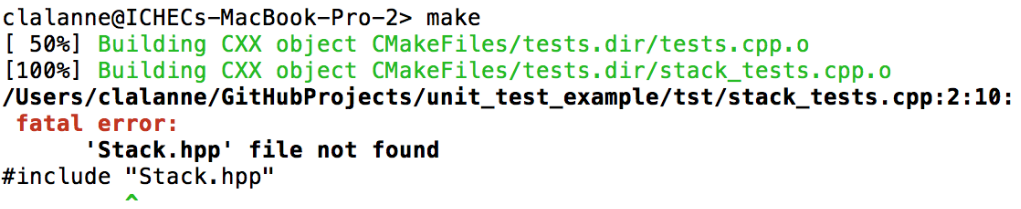
\includegraphics[height=25mm]{\MyFigures/output2.png}\hspace{5mm}
           };
        \end{tikzpicture}
    \end{center}
\end{frame}


\begin{frame}{Primer unit test, implementacion} 
    \inputminted[mathescape,
               linenos,
               numbersep=2pt,
               frame=lines,
               bgcolor=White,
               fontsize=\small,
               linenos,
               framesep=1mm]{c++}
               {\MyCode/stack0.cpp} 
\end{frame}

\begin{frame}{Casi Casi, salida} 
\begin{center}
\begin{tikzpicture}[]
\node[] at (0mm,0mm){
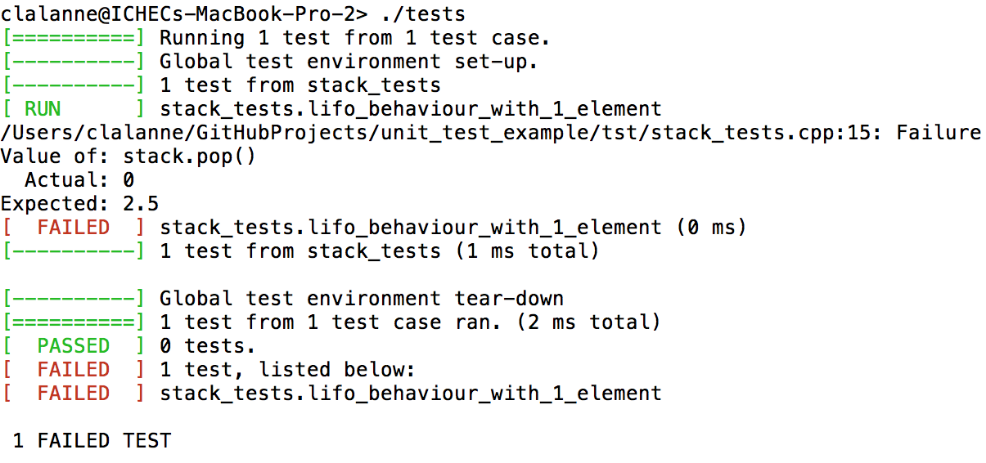
\includegraphics[height=55mm]{\MyFigures/output3.png}\hspace{5mm}
           };
        \end{tikzpicture}
    \end{center}
\end{frame}


\begin{frame}{Creando el primer exito} 
    \inputminted[mathescape,
               linenos,
               numbersep=2pt,
               frame=lines,
               bgcolor=White,
               fontsize=\small,
               linenos,
               framesep=1mm]{c++}
               {\MyCode/stack1.cpp} 
\end{frame}

\begin{frame}{Creando el primer exito, salida} 
\begin{center}
\begin{tikzpicture}[]
\node[] at (0mm,0mm){
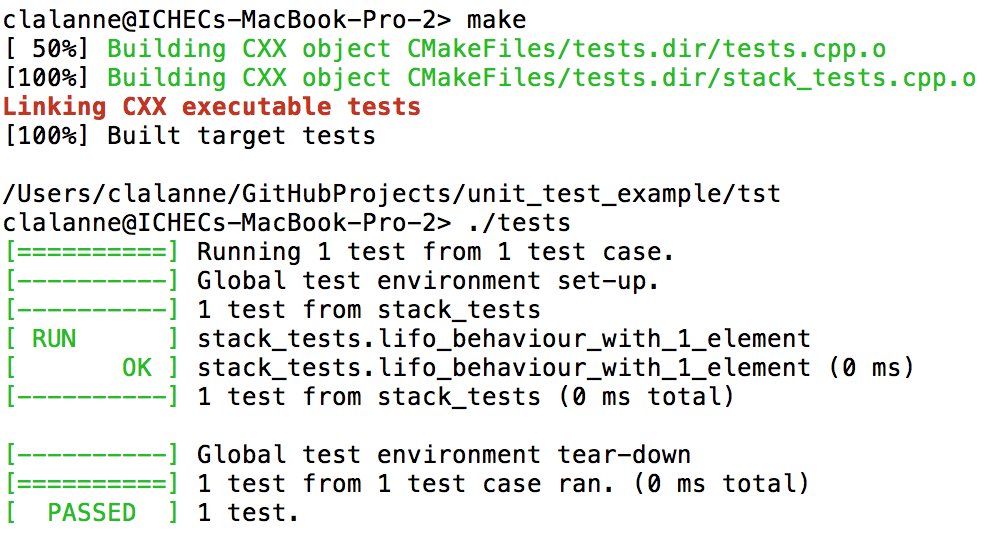
\includegraphics[height=60mm]{\MyFigures/output4.png}\hspace{5mm}
           };
        \end{tikzpicture}
    \end{center}
\end{frame}

\begin{frame}{Algo util} 
    \inputminted[mathescape,
               linenos,
               numbersep=2pt,
               frame=lines,
               bgcolor=White,
               fontsize=\small,
               linenos,
               framesep=1mm]{c++}
               {\MyCode/test1.cpp} 
\end{frame}

\begin{frame}{Algo util, salida} 
\begin{center}
\begin{tikzpicture}[]
\node[] at (0mm,0mm){
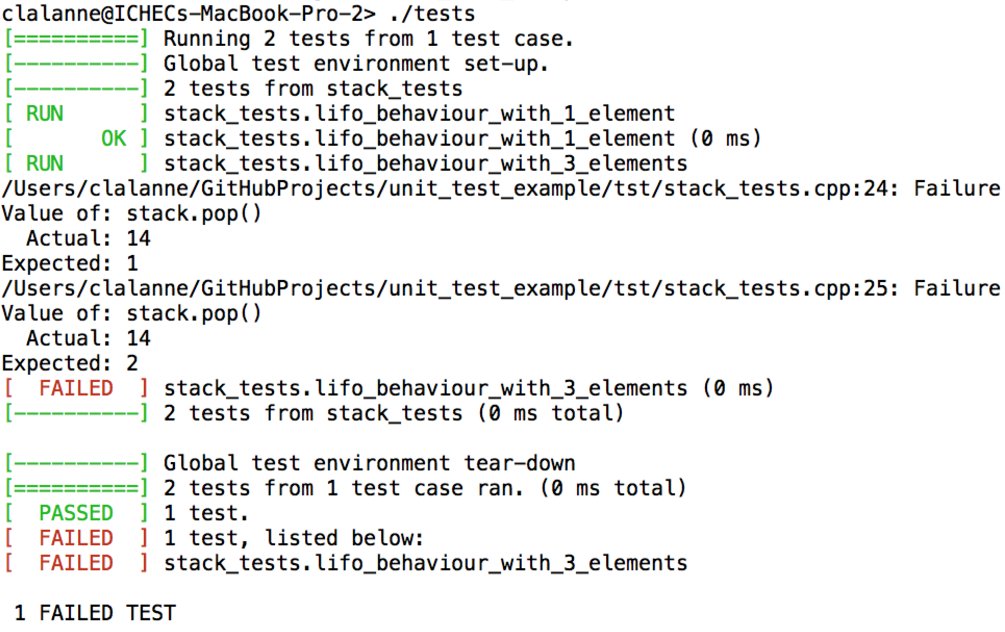
\includegraphics[height=60mm]{\MyFigures/output5.png}\hspace{5mm}
           };
        \end{tikzpicture}
    \end{center}
\end{frame}


\begin{frame}{Algo util, camino al exito} 
    \inputminted[mathescape,
               linenos,
               numbersep=2pt,
               frame=lines,
               bgcolor=White,
               fontsize=\small,
               linenos,
               framesep=1mm]{c++}
               {\MyCode/stack2.cpp} 
\end{frame}

\begin{frame}{Algo util, salida} 
\begin{center}
\begin{tikzpicture}[]
\node[] at (0mm,0mm){
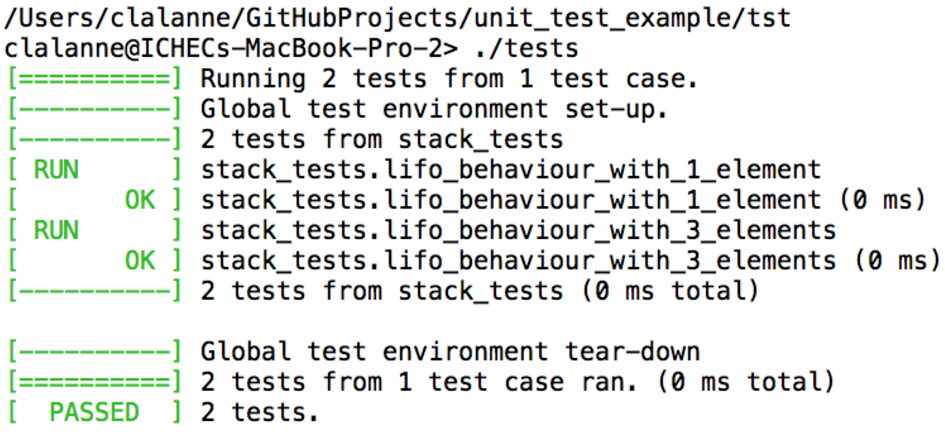
\includegraphics[height=50mm]{\MyFigures/output6.png}\hspace{5mm}
           };
        \end{tikzpicture}
    \end{center}
\end{frame}

\begin{frame}{Biblioteca Stack} 
    \begin{itemize}
        \item Casos bordes
    \end{itemize}
\end{frame}

\begin{frame}{POP de un stack vacio} 
    \inputminted[mathescape,
               linenos,
               numbersep=2pt,
               frame=lines,
               bgcolor=White,
               fontsize=\small,
               linenos,
               framesep=1mm]{c++}
               {\MyCode/emptyStackTest.cpp} 
\end{frame}

\begin{frame}{POP de un stack vacio, salida} 
\begin{center}
\begin{tikzpicture}[]
\node[] at (0mm,0mm){
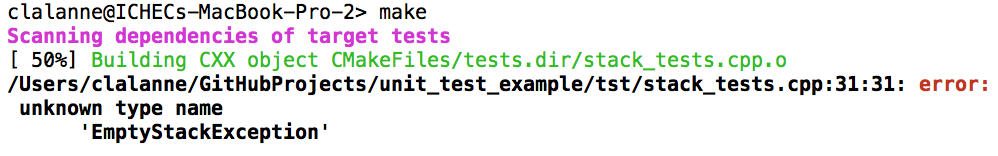
\includegraphics[height=20mm]{\MyFigures/output7.png}\hspace{5mm}
           };
        \end{tikzpicture}
    \end{center}
\end{frame}


\begin{frame}{POP de un stack vacio, implementacion} 
    \inputminted[mathescape,
               linenos,
               numbersep=2pt,
               frame=lines,
               bgcolor=White,
               fontsize=\small,
               linenos,
               framesep=1mm]{c++}
               {\MyCode/EmptyStackException.cpp} 
\end{frame}

\begin{frame}{POP de un stack vacio, salida} 
\begin{center}
\begin{tikzpicture}[]
\node[] at (0mm,0mm){
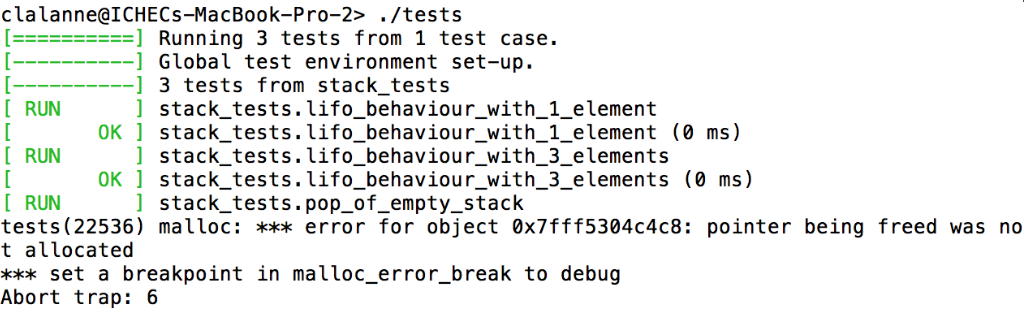
\includegraphics[height=35mm]{\MyFigures/output8.png}\hspace{5mm}
           };
        \end{tikzpicture}
    \end{center}
\end{frame}

\begin{frame}{POP de un stack vacio, implementacion stack} 
    \inputminted[mathescape,
               linenos,
               numbersep=2pt,
               frame=lines,
               bgcolor=White,
               fontsize=\small,
               linenos,
               framesep=1mm]{c++}
               {\MyCode/stack3.cpp} 
\end{frame}

\begin{frame}{POP de un stack vacio, salida} 
\begin{center}
\begin{tikzpicture}[]
\node[] at (0mm,0mm){
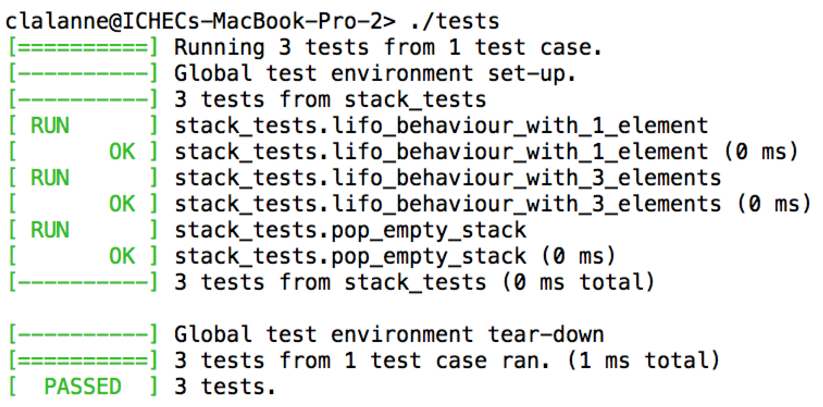
\includegraphics[height=50mm]{\MyFigures/output9.png}\hspace{5mm}
           };
        \end{tikzpicture}
    \end{center}
\end{frame}


\begin{frame}{Mas casos de borde} 
    \begin{itemize}
        \item Limite de tamano de el stack, tiene que ser configurable por el usuario
    \end{itemize}
\end{frame}

\begin{frame}{Tamano configurable} 
    \inputminted[mathescape,
               linenos,
               numbersep=2pt,
               frame=lines,
               bgcolor=White,
               fontsize=\small,
               linenos,
               framesep=1mm]{c++}
               {\MyCode/configurableSizeTest.cpp} 
\end{frame}

\begin{frame}{Tamano configurable, salida} 
\begin{center}
\begin{tikzpicture}[]
\node[] at (0mm,0mm){
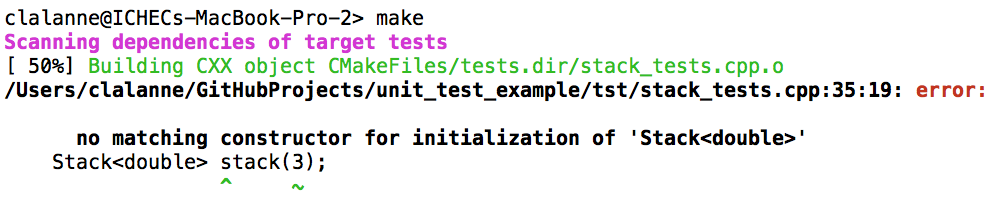
\includegraphics[height=22mm]{\MyFigures/output10.png}\hspace{5mm}
           };
        \end{tikzpicture}
    \end{center}
\end{frame}

\begin{frame}{Tamano configurable, implementacion} 
    \inputminted[mathescape,
               linenos,
               numbersep=2pt,
               frame=lines,
               bgcolor=White,
               fontsize=\tiny,
               linenos,
               framesep=1mm]{c++}
               {\MyCode/stack4.cpp} 
\end{frame}

\begin{frame}{Tamano Configurable, salida} 
\begin{center}
\begin{tikzpicture}[]
\node[] at (0mm,0mm){
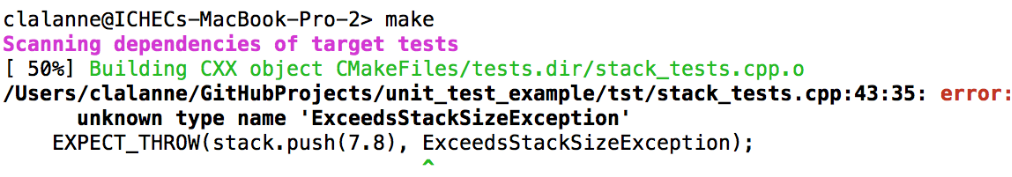
\includegraphics[height=20mm]{\MyFigures/output11.png}\hspace{5mm}
           };
        \end{tikzpicture}
    \end{center}
\end{frame}

\begin{frame}{Excede limite de tamano} 
    \inputminted[mathescape,
               linenos,
               numbersep=2pt,
               frame=lines,
               bgcolor=White,
               fontsize=\small,
               linenos,
               framesep=1mm]{c++}
               {\MyCode/ExceedsStackSizeException.cpp} 
\end{frame}

\begin{frame}{Tamano Configurable, salida} 
\begin{center}
\begin{tikzpicture}[]
\node[] at (0mm,0mm){
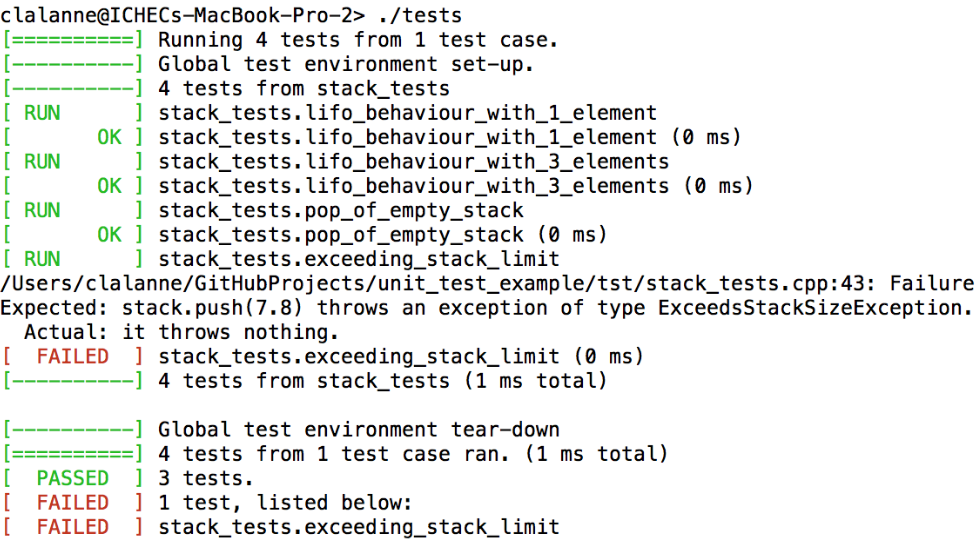
\includegraphics[height=50mm]{\MyFigures/output12.png}\hspace{5mm}
           };
        \end{tikzpicture}
    \end{center}
\end{frame}

\begin{frame}{Codigo final} 
    \inputminted[mathescape,
               linenos,
               numbersep=2pt,
               frame=lines,
               bgcolor=White,
               fontsize=\tiny,
               linenos,
               framesep=1mm]{c++}
               {\MyCode/stack5.cpp} 
\end{frame}

\begin{frame}{Codigo final, salida} 
\begin{center}
\begin{tikzpicture}[]
\node[] at (0mm,0mm){
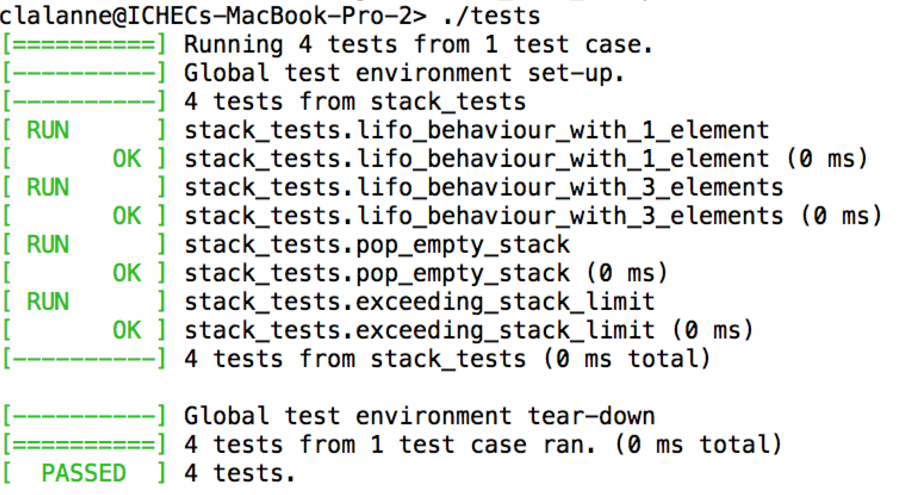
\includegraphics[height=50mm]{\MyFigures/output13.png}\hspace{5mm}
           };
        \end{tikzpicture}
    \end{center}
\end{frame}

\begin{frame}{Todos los tests} 
    \inputminted[mathescape,
               linenos,
               numbersep=2pt,
               frame=lines,
               bgcolor=White,
               fontsize=\tiny,
               linenos,
               framesep=1mm]{c++}
               {\MyCode/allTests.cpp} 
\end{frame}

\begin{frame}{Ciclo TDD}
\begin{center}
\begin{tikzpicture}[]
\node[] at (0mm,0mm){
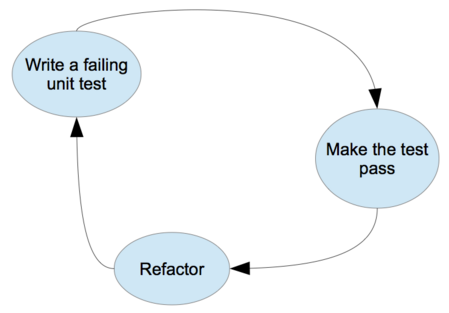
\includegraphics[height=40mm]{\MyFigures/tddCycle.png}\hspace{5mm}
           };
        \end{tikzpicture}
    \end{center}
\end{frame}

\begin{frame}{Test Driven Development} 
    \begin{itemize}
        \item Rapida y continua retro-alimentacion
        \item TDD abilita refactoring
        \item Lecciones aprendidas, experiencias ganadas no se pierden, quedan en los tests
    \end{itemize}
\end{frame}


\begin{frame}{Test Driven Development} 
    \begin{itemize}
        \item TDD nos da retroalimentacion de:
        \begin{itemize}
            \item El codigo esta funcionando?
            \item El codigo esta bien disenado?
        \end{itemize}
    \end{itemize}
\end{frame}

\begin{frame}{Test Driven Development} 
    \begin{itemize}
        \item Escribir los tests nos da:
        \begin{itemize}
            \item Clarificar el criterio de aceptacion de nuestra proxima unidad de codigo
            \item Alta cohesion y bajo aclopamiento, para probar unidades de forma facil
            \item Descripcion ejecutable de lo que el codigo hace
            \item Unit tests
        \end{itemize}
    \end{itemize}
\end{frame}

\begin{frame}{Test Driven Development} 
    \begin{itemize}
        \item Ejecutar los tests nos da:
        \begin{itemize}
            \item Detectar errores cuando el conocimiento de el contexto esta en mente aun fresco
            \item Nos deja saber cuando estamos listos, evita sobre implementar/sobre generalizar features
        \end{itemize}
    \end{itemize}
\end{frame}

\begin{frame}{Test Driven Development} 
    \begin{itemize}
        \item Esto trae consigo desarrollo de software incremental e iterativo
    \end{itemize}
    \begin{itemize}
        \item Nunca escribir una nueva funcionalidad sin primer tener un test que falle
    \end{itemize}
\end{frame}


